\section{Hardware}
\label{sec:pastwork:hardware}

% ~\cite{Li:2011ur,Li:2010en,Zhang:2009dp}

Different approaches are available for 3D imaging including laser scanning~\cite{Blais:1988te}, viewpoint reconstruction~\cite{Hartley:2000un} and structured light scanning~\cite{Halioua:1984ue}. Structured light scanning, compared to other approaches, is fast and accurate. For palmprint recognition, speed is an important factor. The verification or identification result must be given in a short time. Otherwise the system is barely suitable for real-world applications.

% http://en.wikipedia.org/wiki/Structured-light_3D_scanner

Projecting a narrow band of light onto a three-dimensionally shaped surface produces a line of illumination that appears distorted from other perspectives than that of the projector, and can be used for an exact geometric reconstruction of the surface shape (light section).

A faster and more versatile method is the projection of patterns consisting of many stripes at once, or of arbitrary fringes, as this allows for the acquisition of a multitude of samples simultaneously. Seen from different viewpoints, the pattern appears geometrically distorted due to the surface shape of the object.

\begin{figure}[htb]
  \begin{center}
    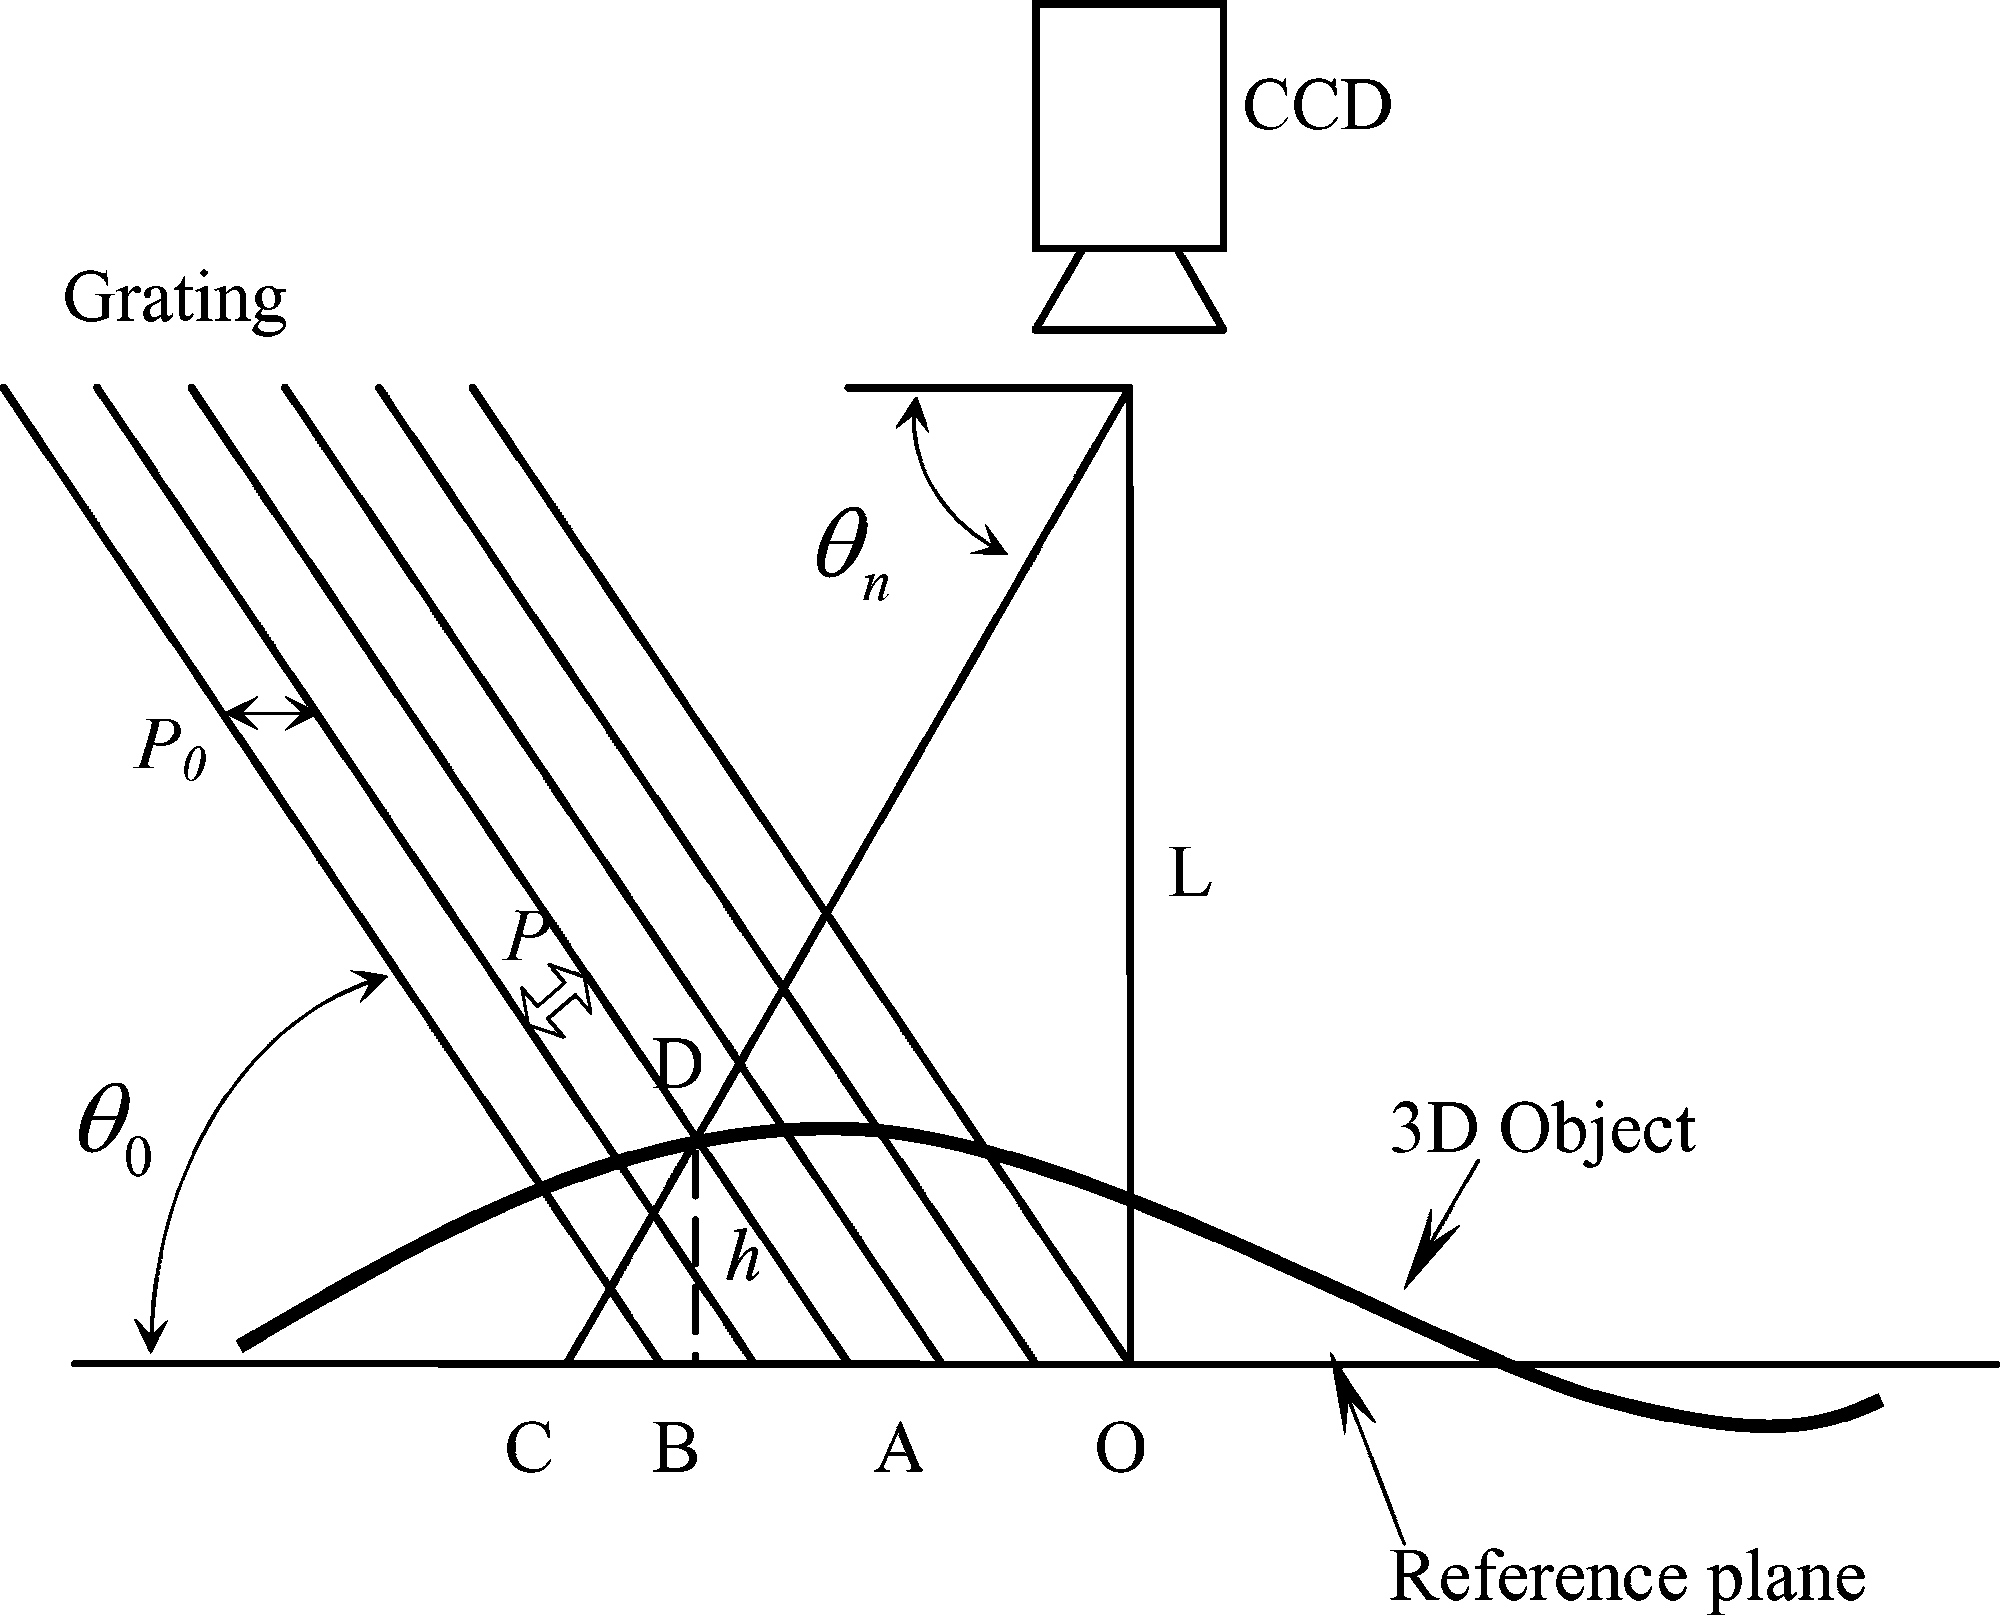
\includegraphics[width=0.9\linewidth]{ch-pastwork/figures/sli}
    \caption[The principle of structured-light imaging]{The principle of structured-light imaging\cite{Li:2009eq}}
    \label{fig:pastwork:sli}
  \end{center}
\end{figure}

Although many other variants of structured light projection are possible, patterns of parallel stripes are widely used. Figure~\ref{fig:pastwork:strippattern} shows the geometrical deformation of a strip pattern projected onto a palm. The displacement of the stripes allows for an exact retrieval of the 3D coordinates of any details on the palm's surface.

David et. al designed a 3D palmprint capturing device~\cite{Zhang:2008kc}. The system proposed has a resolution of 768x576.

\begin{figure}[htb]
  \begin{center}
    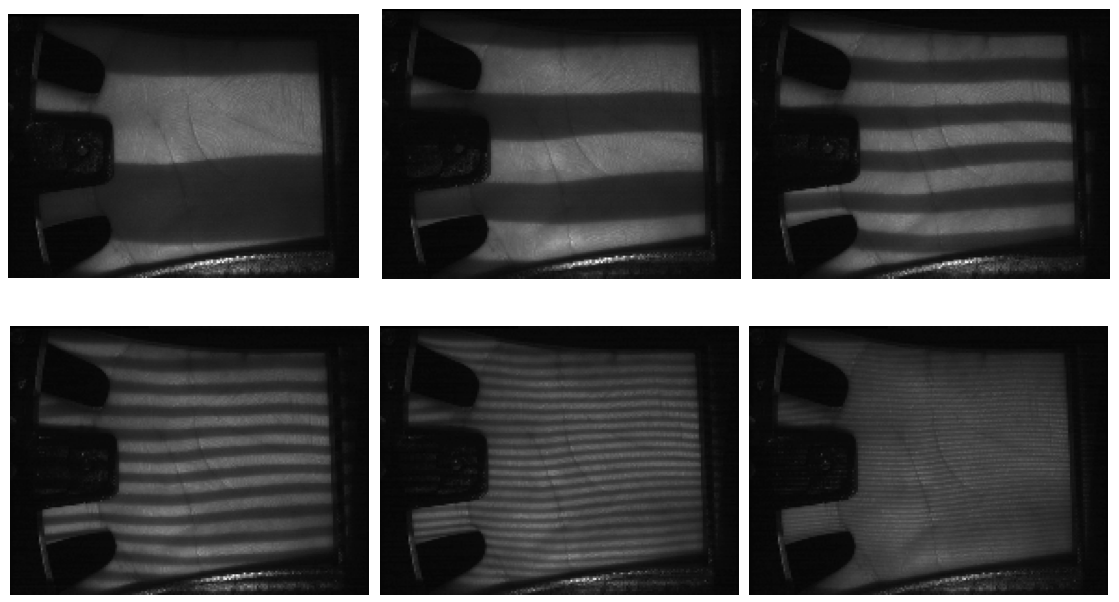
\includegraphics[width=0.9\linewidth]{ch-pastwork/figures/strippattern}
    \caption[Sample patterns of the stripes on the palm]{Sample patterns of the stripes on the palm~\cite{Li:2009eq}}
    \label{fig:pastwork:strippattern}
  \end{center}
\end{figure}
